% Chapter Template

\label{chpt:introduction} % for referencing this chapter elsewhere, use \ref{chpt:label}
\lhead{\emph{Background, context, and motivation}} % This is for the header on each page - perhaps a shortened title

% Here, re-write and update the first year literature review. re-contextualise it in the narrower scope of AML, which I ended up actually doing.

Cataclysmic Variable (CV) systems consist of a white dwarf primary, and a lower mass red dwarf secondary star. The two are in extremely close proximity, such that the outer layers of the secondary are gradually accreted onto the white dwarf; this mass transfer process affects the evolution of both stars, in particular the donor, and is the main driving mechanism for the evolution of the system as a whole.
The accretion also gives two further key features of a CV: an accretion disc around the white dwarf, and a shock-heated bright spot region where accreted donor material impacts the outer rim of the disc\todo{Do I really need a reference for this? Probably just reference that "on cataclysmic variables" or whatever that book was. You know the one.}\todo{Put in your CV schematic here. Maybe update it and try to make it prettier?}.
Systems actively undergoing mass transfer are important to our understanding of stellar evolution, as a diversity of stars will experience a mass transfer phase, and losing mass strongly influences a stars' evolutionary path and must be accounted for. Of such systems, CVs in particular are interesting as modelling their eclipse lightcurves can yield precise, independent measures of both stars' mass and radius \citep{wood1986, Littlefair2008, Savoury2011}. Further, since the donor stars' evolution is completely dominated by its mass loss, CVs provide a window into binary evolution \citep{knigge2006}.

Since CVs involve poorly understood physics, such as magnetism and the structure and evolution of low mass stars, but are also open to comprehensive analysis, they provide an excellent test-bed for binary evolution modelling, and the difficult processes that contribute to them. Unfortunately, whilst modelling most of a CV's life is now possible \citep{Paxton_2015}, the field has yet to produce physically motivated models capable of accurately reproducing either the CV population distribution, or complete evolutionary track, indicating some shortfalls in our understanding\todo{ref here - was it a savoury paper? Perhaps pala? I cant remember}. Of most significance to this work is the problem of missing Angular Momentum Loss (AML), where CVs with extremely low mass donor stars appear to be losing angular momentum much faster than our models predict\todo{ref}. This first chapter will summarise the current understanding of CV formation and evolution, and the current state of CV modelling. 

The bulk of this thesis is focused on two elements: firstly, the sample of well-characterised (i.e. measured masses and radii for both stars, white dwarf temperature and surface gravity, orbital period, and inclination) eclipse modelled CVs is small - only 18 systems prior to this work. I characterise an additional XXX systems\todo{Put in here how many systems}. While this is still a small sample, it is now enough for approximate statistical analysis. Second, using stellar models, I affirm the observations\todo{cite this} that the canonical CV evolutionary track fails at periods shorter than $\sim 2.5$ hours, and produce an empirical correction to predicted AML, as a function of donor mass. Through this, I hope to constrain the possible sources of missing AML. 

\section{Roche geometry}
\label{sect:introduction:Roche geometry}
\todo{Proof read this section}

Before discussing the formation, structure, and evolution of CVs, it is critical to understand Roche lobes.
In a two-body orbital system, the Roche potential of a point is an effective potential in the non-inertial, co-rotating frame of reference. It is given by the sum of the gravitational potential energies due to the two masses, and the potential energy arising from centrifugal force. This can be described mathematically for each position vector:
\begin{equation}
    {\bf \phi} = -\frac{G M_1}{|{\bf r - r}_1|} - \frac{G M_2}{|{\bf r - r}_2|} - \frac{1}{2}({\bf \Omega} \times {\bf r})^2
\end{equation}
Where $\phi$ is the Roche potential, G is the gravitational constant, $\bf r$ is the position vector being considered, and $\bf \Omega$ is the angular momentum vector of the binary. $M_{1,2}$ and ${\bf r}_{1,2}$ are the masses and position vectors of the two orbiting bodies.

\begin{figure}
    \centering
    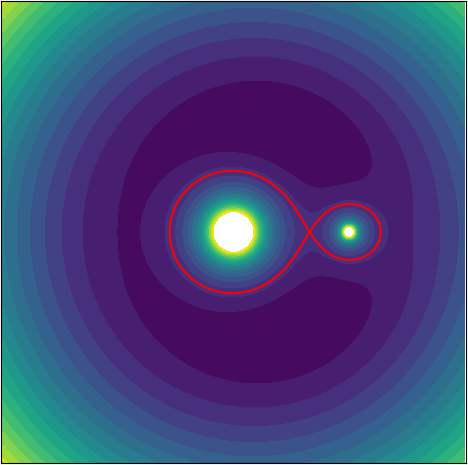
\includegraphics[width=\columnwidth, trim={0mm 0mm 380px 0mm}, clip]{figures/introduction/roche.png}
    \caption{Showing the Roche potential in the neighbourhood of the binary system. Each line represents a line of equipotential. Taken from \citet{cerutti2007}}
    \label{fig:roche}
\end{figure}

Near to each of the bodies, the gravitational potential is large and negative, and dominates the Roche potential. This becomes \textit{less negative} as we move away from that body. Conversely, angular momentum is less negative closer to the center of mass, and more negative as we move away from the system and larger velocities are required to co-rotate. Broadly, there are then three regimes: a very negative Roche potential near each of the two bodies, a less negative region immediately surrounding the two bodies, and a very negative region far from the two bodies. The overall potential is smooth, so joining the three regions requires a ridge encircling the orbiting bodies, and a saddle between them. Figure~\ref{fig:roche}\todo{Make your own version of this figure - this one is blurry and ugly} shows this graphically. The saddle is centred on the first Lagrangian point, $L_1$, and is the point at which a small (co-rotating) mass is attracted equally and oppositely by both bodies. We can trace the line of constant potential that passes through the $L_1$ point, giving two teardrops joined at the tips. The teardrop that encapsulates a star is known as its Roche lobe. Matter that extends beyond the Roche lobe is no longer gravitationally bound to its parent body, and will either fall onto its companion via the $L_1$ point, or otherwise be ejected from the star. This material will no longer be in a stable orbit, so will either be ejected from the system, or find a new higher orbit where the two-body effects are negligible.

The shape of the Roche lobes are non-trivial to calculate, and must be done numerically. However, approximations exist for the volume-equivalent radius of a Roche lobe (that is, the radius of a sphere of equivalent volume). Most commonly used is the \citet{Eggleton1983} approximation,
\begin{equation}
    \label{eqn:eggleton approximation}
    \frac{R_L}{a} = \frac{0.49 q^{2/3}}{0.6 q^{2/3} + \mathrm{ln}(1 + q^{1/3})}
\end{equation}
where $a$ is the orbital separation, and $q$ is the mass ratio of the system, $M_2 / M_1$. In CVs, where the secondary star is completely filling its Roche lobe, $R_L$ makes for a good approximation for the secondary stars' radius.

\section{CV formation}
\label{sect:introduction:formation of CVs}

The formation of a CV begins with a binary system forming at a distance of $\sim 100{R_\odot}$. Crucially, the stars differ significantly in mass, one typically being $<1{M_\odot}$ and the other $>1{M_\odot}$ \citep{Ritter2012}. The lifespan of a star falls as its mass increases, so the larger star evolves faster than its companion, ascending the red giant branch after a few Gyrs and expanding to fill its Roche lobe. 
As the outer layers contact the Roche lobe, stellar material crosses the boundary between being gravitationally bound to the donor and being ejected from its surface. 
Once the outer layers of the primary contact the Roche lobe, the $\mathrm L_1$\ point forms a locus for mass to move from the massive, evolved star onto the less evolved secondary star.

As mass moves away from the primary, and away from the centre of mass of the system, it gains angular momentum. However, because angular momentum is conserved within the binary this is offset by a drop in separation, $a$, and the radius of the Roche Lobe, ${R_L}$, contracts. \textit{More} matter is now outside the primary Roche lobe, encouraging further mass transfer and hence further reduction in orbital separation \citep{Ritter2008}.

With this positive feedback loop, the primary can rapidly transfer its whole envelope, though the transfer rate $\dot M$ is too high to for all of this to be properly assimilated into the primary surface. The process is very rapid -- so rapid that models have been unable to properly resolve it, but is probably $\sim 10^2 - 10^3$ years in duration \citep{Ritter2012}. With this influx of mass, the secondary star grows and the accreted matter forms a thick, bloated, and deeply convective envelope on the star. The increased radius of the secondary brings the two bodies into contact \citep{Ritter2008} and the stars enter a common envelope phase of evolution. See \citet{paczynski1976} for an original reference on common envelope evolution, or \citet{ivanova2020} for a recent review of the topic. For detail on this phase as it relates to CVs, see \citet{taam1978, webbink1984, zorotovic2010, passy2011}.

The common envelope phase transfers much of the secondary stars' angular momentum to the shared envelope, though the mechanism for this is poorly understood \citep{demarco2011}. If the common envelope is substantial enough, the reduction in separation between the two stellar cores can be completely reduced, and the two merge together. If it is not, the entire envelope is stripped from the stars, and the two are left in a compact orbit. CV systems are the product of the latter scenario - the common envelope is ejected via a strong wind, leaving the remnant core of the primary as a white dwarf, and a low mass secondary companion M dwarf. 

The common envelope phase can be parameterised with the energies involved, namely the gravitational binding energy of the envelope, $U_{\rm bind}$, and the change in the angular momentum contained in the orbit before and after the common envelope phase, $\Delta U_{\rm orb}$, as the common envelope efficiency parameter, $\alpha$.
\begin{equation}
    \alpha = \frac{U_{\rm bind}}{\Delta U_{\rm orb}}
\end{equation}
This is known as the $\alpha$ formalism \citep{demarco2011}, and is a good illustration of how poorly we understand CE evolution. $\alpha$ should be a metric we can predict with models, but this has proven very challenging and several competing frameworks exist \citep{ivanova2020}. 

The energy needed to liberate the envelope is expected to come from the angular momentum of the binary, but some systems have been observed and characterised with $\alpha > 1$. This suggests that other sources, like the thermal output of the stars, contributes to the envelope ejection \citep{demarco2011, ivanova2013}. Common envelope evolution remains a very difficult problem to solve, and only approximate models currently exist \citep{ivanova2020}, but the following scenario is generally accepted as likely in the case of CVs.

During the common envelope phase, the envelope is expelled into a planetary nebula \citep{Ritter2012}, and $\alpha$ in the case of a proto-CV hass been loosely estimated to be $\sim 0.2 - 0.6$ \citep{politano2007}, and some evidence exists for lower $q$ systems having larger $\alpha$\citep{passy2013}. The ejecta carries with it angular momentum, causing $a$ to quickly fall from $\sim 100 R_\odot$ to less than $1 R_\odot$\todo{cite}, leaving behind a white dwarf and a low mass companion star -- usually a cool, red M dwarf -- in an extremely compact orbit, typically a few \Rsun. At this point, the red dwarf detaches from its Roche lobe and mass transfer is shut off. Angular momentum is shed through magnetic braking and gravitational wave braking until the donor comes into contact with its Roche lobe. Mass transfer can then resume, though this time in the more stable secondary-to-primary direction. The system is now a CV, and its evolution from here will be dominated by AML and mass transfer, detailed in \S\ref{sect:introduction:AMLMechs}.


\section{CV evolution}
\label{sect:introduction:Summary of how AML and Mdot drive period evolution}

Initially, mass from the more massive star transferred to the smaller one, but once the system emerges from the common envelope phase, AML causes the orbit to tighten until the less massive red dwarf secondary fills its Roche lobe. This now means that mass transfer is moving matter closer to the system's centre of mass, imparting angular momentum to the secondary as it does so. This causes the donor to retreat, and increases $R_L$. Hence, mass transfer now acts to decrease further transfer \citep{Ritter2008}, rather than exacerbate it.

To resume mass transfer some mechanism is necessary to shed angular momentum and bring the secondary back in contact with its Roche lobe. 
Canonically, two mechanisms are thought to drive this; gravitational wave braking, and magnetic braking.
AML drives the two bodies closer together and triggers mass transfer, and mass loss from the donor drives it to retreat from the white dwarf primary. These two processes find equilibrium when the donor is just barely overflowing its Roche lobe, and the angular momentum gained by the donor from mass transfer is offset by the AML from the system.
The mass transfer timescale of the donor is much shorter than its nuclear timescale, so mass loss dominates its evolution and gives rise to a single, unified CV evolutionary path.

There is a further complicating factor to consider; while the secondary is losing mass, it is not in thermodynamic equilibrium. The outer layers are being lost, which reduces the pressure on the core and so reduces the rate of fusion. 
The thermal timescale is much longer than the mass loss timescale, so the star is unable to cool and contract to its equilibrium radius. This leaves the star hotter than it would be under zero mass loss, and so its radius increases in response to the mass loss, and a higher mass loss rate results in larger inflation.
When the donor first connects to its Roche lobe, this causes an initial spurt of mass loss and an increase in orbital period, but reconnection quickly reoccurs and remains stable. 


\subsection{Sources of angular momentum loss}
\label{sect:introduction:AMLMechs}

When two bodies orbit each other in space, the periodic warping of space-time produces gravitational waves. These waves carry energy away from the system, robbing it of angular momentum and reducing the orbital radius \citep{Paczynski1967}. In CVs, the rate of momentum loss from gravitational waves is small, so long timescales (by human standards) are needed to significantly alter the orbital period, $P$.
The rate of change of the period, $\dot P$, should be possible to probe with long-baseline observations (e.g. \citealt{qian2007, shafter2021}), but are prone to large errors and are difficult to gather data for. However, this has not prevented some systems having their $\dot P$ inferred indirectly and a few such characterisations have been done. Notably, \citet{pala2020} recently inferred the mass loss rates (which directly relates to $\dot P$) of 42 CVs from HST spectra, using the white dwarf temperature and mass as diagnostics. 
\todo{Stu disagrees - update your understanding here.}In the near future, CV gravitational waves are expected to be visible to the LISA mission, and direct measurements of $\dot P$ at scale will become feasible \citep{Meliani2000, kalomeni2016}. 

Population synthesis models do not match observations with gravitational braking alone, and magnetic braking is thought to make up the deficit (e.g. \citet{kolb1993a, kolb1993, Davis2008, garraffo2018}).
Additionally, \citet{Townsley2009}, \citet{Pala2021} infer the mass transfer rate (a diagnostic of $\dot P$) from the white dwarf surface temperature, and find results inconsistent with pure gravitational braking.

If one of the stars has a strong magnetic field (often assumed to be the secondary, though white dwarfs can have strong `frozen-in' magnetic fields \citep{TOUT2011}), any wind emanating from the system, which is made up of charged particles, and likely originating from the secondary, will couple with the magnetic field to some degree and carry some angular momentum away from the binary with it.
In the case of a CV, the wind originates from the secondary star, and the magnetic field is often assumed to be associated with the secondary also, though white dwarfs can have strong `frozen-in' magnetic fields \citep{TOUT2011}.

\todo{Is this wise? I think it's a catch 22 - I need MB to explain CV evolution, but I need to have talked about the long-P, Pgap, and short P CVs to really get into the MB weeds...}A detailed description of the modern understanding of magnetic braking is given in \S\ref{sect:introduction:magnetic braking}, after the following outline of CV evolution. Some elements of CV evolution are necessary to understand magnetism in CVs.



\subsection{Period evolution and key population features}
\label{sect:introduction:period distribution key features}
\begin{figure}
    \centering
    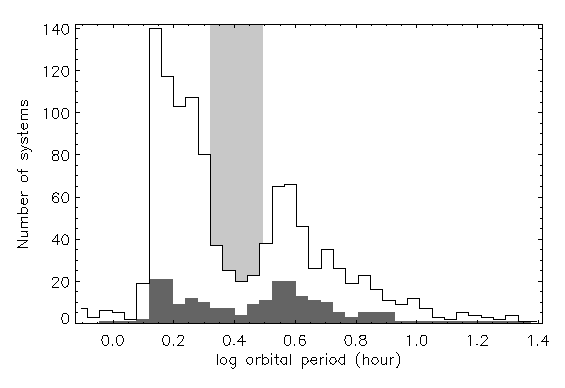
\includegraphics[width=\columnwidth]{figures/introduction/pd-rk.eps}
    \caption{Reproduced from \citet{southworth2015}, Figure~14. The orbital period distribution of RKCat \citep{RKCat} CVs identified by the SDSS (white histogram) and of the subset of these which are eclipsing (grey histogram). The light grey rectangle delineates the period gap at 2.1–3.1 hours. The periods have been collected into histogram bins which are of equal size in log space.}
    \label{fig:period hist}
\end{figure}

Through careful observation, The orbital period of a CV can be measured by tracking either their spectroscopic radial velocities (e.g. \citealt{gaensicke2009}), or the timings of repeating features in their lightcurves (e.g. \citealt{Littlefair2008}). Once this has been done for a large enough sample, a histogram of the periods can be plotted. This plot, shown in fig.~\ref{fig:period hist}, is important to understanding how a CV will evolve over time.
There are three immediately obvious features of the plot;
\begin{itemize}
    \item a long period cutoff, as the number of systems taper off after $\sim12$hrs
    \item a period gap at $\sim2-3$hrs
    \item a period minimum at $\sim1$ hour, with a pile-up of systems just above it.
\end{itemize}
Each of these features are discussed in turn.

\subsection{The period maximum}
\label{sect:introduction:period maximum}
In order for a system be be a CV, mass must be transferring from a less massive star, onto a compact object, constraining the maximum value of $q$ to $\sim1$, and demanding that the secondary extends out to $\sim R_L$. 

There are two immediately obvious constraints for a CV. The mass ratio, $q = \frac{M_{\rm donor}}{M_{\rm WD}}$, must be less than 1 for stable mass transfer, and the donor radius must be approximately equal to the Roche radius.
An additional constraint is that the maximum mass of a white dwarf is well known to be limited to $\le 1.4M_{\odot}$ before triggering thermonuclear runaway \citep{chandrasekhar1942}.

An important feature of a Roche lobe is that for a fixed mass ratio, $q=\frac{M_1}{M_2}$, its radius, $R_L$, is roughly linearly dependant on the orbital separation, $a$. Recall the Eggleton approximation for a Roche lobe radius, Equation~\ref{eqn:eggleton approximation}:
\begin{equation}
    \tag{\ref{eqn:eggleton approximation}}
    \frac{R_L}{a} = \frac{0.49 q^{2/3}}{0.6 q^{2/3} + \mathrm{ln}(1 + q^{1/3})}
\end{equation}

\citet{warner1995} found that the average density, $\rho_{av}$, for objects that fill their $R_L$ follows a robust relationship;
\begin{equation}
    \frac{\rho_{av}}{\rho_{\odot}} = 75.9 P_{orb}^{-2}(h)
\end{equation}
\citet{knigge11} derived a connection between CV secondary mass and radius, $M_2$ \& $R_L$. This can be manipulated to produce a mass-period relationship,
\begin{align}
    \rho_{av} = \frac{3 M_2}{4 \pi R_L^3} &\simeq 75.9 P(h)^{-2} \\
    \frac{R_L}{R_\odot} = C &\cdot \Big( \frac{M_2}{D \cdot M_\odot} \Big) ^{\alpha}
\end{align}
where $C$ and $D$ are constants for a particular regime, i.e., short-period, long-period, or period bouncer, and $\alpha$ is the mass-radius index \citep{Knigge2011b}.
Combining the above gives a pleasingly simple relationship.
\begin{equation}
\label{eqn:MP_relation}
    M_2^{(1-3\alpha)} \propto P^{-2}
\end{equation}

For long-period CVs, $\alpha = 0.67\pm0.04$ \citep{knigge11}, and equation \ref{eqn:MP_relation} becomes $M_2^{1.01} \propto P^{2}$, and larger secondary masses require longer periods. The theoretical maximum secondary mass of $1.4 M_{\odot}$ corresponds to a period of $\sim12$hrs, though in reality these higher masses are rarer and the frequency of CVs at these higher periods begins to drop much earlier, at $\sim6$hrs \citep{gaensicke2009}. Note while the above is specific to long-period systems, and $\alpha$ is a non-linear function of mass, and different values are needed for the period gap and short period regimes.


\subsection{The period gap}
\label{sect:introduction:period gap}

Between periods of around 2-3 hours, there is a dramatic fall in the number of CVs we detect. Volume-limited samples indicate that this is a real effect and not a selection bias \citep{Kolb1998}. However, the origin of this gap in the period is something of an open problem.

Models indicate that long period systems ($P > 3$h) have far higher mass loss rates than short period systems ($P < 2$h) \citep{ritter1985}. This suggests a significant change in braking mechanisms between the two regimes. 

The disruption of magnetic braking was proposed early on to explain the period gap \citep{rappaport1983, spruit1983}, and relatively shortly after \citet{kolb1993} showed more quantitatively that a sub-class of purely gravitational braking CV systems does not reproduce the observed population. Historically, the standard evolutionary path of CVs has involved the secondary becoming fully convective which was thought to disrupt the magnetic field and so cease MB \citep{knigge11}, though this has frequently been questioned. \todo{Gather references}

It is important to develop diagnostics for the nature of the period gap, and \citet{smith1998} show how spectral analysis could yield an accurate observed mass-radius relation for donor stars in CVs as evidence for MB, though they lacked the observations to apply their method. The mass-radius relation would later be carried out by \citet{knigge11}.
\citet{Davis2008} used population synthesis to demonstrate that, if the period gap is caused by disrupted MB, this may affect the mass function of quiescent CVs that are moving through the gap. They expect an excess of non-transferring CVs over low mass post-common envelope CVs that emerge from the common envelope phase directly into the period gap. These should form at a predictable rate across $q$, but due to the slow crossing of quiescent CVs, the latter `pile up' in the gap - a detectable effect observed by \citet{zorotovic2011}.

Disrupted MB has faced some difficulty in recent years. X-ray emission level is a diagnostic of magnetic flux \citep{pevtsov2003}, and \citet{wright2016} found that the X-ray flux of CVs is similar between fully convective and non-convective main-sequence stars, implying a similar magnetic field strength. Furthermore, disagreement between observational and theoretical period gap and minimum locations \citep{knigge11} has left the disrupted MB model an area of active research. 
\citet{garraffo2018} recently proposed that the magnetic field does not weaken, but rather becomes more complex which reduces the efficiency of MB. If this disruption does occur, the secondary can now contract on to its equilibrium radius, and quickly disconnects from its Roche lobe. The system then becomes quiescent, no longer presenting as a CV, but rather as an inert binary. As such, it is no longer included on the CV period diagram, and so the upper edge of the period gap develops.

The system is still subject to gravitational radiation, however, so gradually evolves back towards shorter periods. Once the secondary reconnects with its Roche lobe, mass transfer resumes and the system again presents itself as a CV, emerging from the period gap at a $\sim2$hr period \citep{kolb2002}.

\subsection{The period minimum, and period bouncer systems}
\label{sect:introduction:period minimum and bouncers}

The period minimum was first predicted by \citet{rappaport1982}, and can be understood by considering the two governing timescales affecting the secondary. 
For donors with masses above $\sim0.1 M_{\odot}$, the donor is contracting in response to mass loss. However, at a period of about 80 minutes \citep{ritter1998, McAllister2019}, $\tau_{\dot M}$ becomes longer than $\tau_{therm}$, causing the donor to lose mass adiabatically and expand rather than contract. This now allows the donor to remain in contact with its Roche Lobe when mass loss raises it to a higher orbit, and the system evolves to longer periods over time.

More quantitatively, as the components of a short period CV move closer together and the donor falls in mass, $\tau_{therm}$ and $\tau_{\dot M}$ become more out of balance, corresponding to $\alpha$ in equation \ref{eqn:MP_relation} decreasing \citep{Knigge2011b}. A main-sequence star will have $\alpha \sim 1$, but a secondary subjected to fast, adiabatic mass loss will have $\alpha \simeq -1/3$. Looking at the gradient of equation \ref{eqn:MP_relation}, the existence of a period minimum can be easily seen.
\begin{equation}
    \frac{\dot P}{P} = \frac{(3\alpha - 1)}{2} \frac{\dot M_2}{M_2}
\end{equation}
When $\alpha \le 1/3$, a negative $\dot M$ will produce a \textit{positive} change in $P$, and the donor begins to retreat from the white dwarf \citep{rezzolla2001}. 

This has been confirmed by \citet{knigge11}, who found that for period bouncer CVs, $\alpha = 0.21^{+0.05}_{-0.10}$, giving the following empirical version of equation \ref{eqn:MP_relation} in the post-period minimum regime.
\begin{align}
    M_2 \propto P^{-5.4}
\end{align}

\todo{First-pass proof read up to here}


\section{Magnetic Braking}
\label{sect:introduction:magnetic braking}

\todo{Fill in some more stuff. You have some points in the "problems with modelling" bit later.}

Consider a blob of this charged wind material, moving with some sideways velocity in the plane of the orbit, almost certainly slower than the magnetic field lines. 
The blob will interact with the field and accelerated to co-rotate with them.
This higher velocity causes it to move outwards, to a higher orbit, where the field lines are moving even faster, accelerating the blob more. 
The wind then robs the star associated with the magnetic field of rotational angular momentum and its spin rate is slowed. The close proximity of the binary means that tidal effects are strong, and the donor is spun up again by robbing the orbit of angular momentum, reducing their separation and hardening the binary further \citep{verbunt1981}.

As an aside, \citet{wickramasinghe1996} presented theoretical motivation that CVs can have too strong a magnetic field to allow magnetic braking. Open field lines are necessary for wind to escape the system, so too strong a white dwarf magnetic field can trap the ionised gas in-system, suppressing the wind of the secondary. This Magnetic CV subclass is briefly described in \S\ref{sect:introduction:magnetic CVs}.

As the magnetic braking mechanism is a direct consequence of the donor star spinning down, the CV community is able to borrow insights from adjacent fields of study. The majority of M dwarfs experience some form of spin-down under magnetic braking \todo{cite this}, so observations of the magnetic field strengths of singletons should inform the efficacy of magnetic braking in CV binaries\todo{reference this}. Unfortunately, the typical CV rotational period is on the order of a few hours, and singleton M dwarfs are considered extremely fast rotators with periods of a day\todo{Cite this}. Observations of singletons simply do not reach to the extremely low mass, rapid rotations that are frequently seen in CVs, so we are forced to rely on extrapolation and theory.

This carries with it some major practical issues. One is that while the broad effects of magnetic fields is relatively easy to intuit, quantitative physical understanding the mechanics and origins of magnetic fields is difficult, involving fluid dynamics, considering interactions with the accretion disc, and magnetism acting on large systems, which quickly become prohibitive to model and is usually handled with one of a variety of recipes. \citealt{knigge11} contains a detailed compilation of some older approaches, but the decade since has seen a few newer methodologies emerge. Here, a brief description of two recent magnetic braking prescriptions: the \citet{matt2015} prescription, and the \citet{garraffo2018a} prescription. However, for a detailed summary of the modern understanding of M dwarf magnetic fields refer to \citet{kochukhov2021}. 

\subsection{Mass dependant angular momentum loss}

In \citet{matt2015}, an empirical prescription is derived that relates the torque felt by a low mass main sequence star to that stars' mass, radius, and Rossby number. The Rossby number is a fluid dynamics term for the ratio between the inertial and Coriolis force terms of the Navier-Stokes equations. A small Rossby number indicates a system dominated by Coriolis effects, and a large Rossby number indicates that centrifugal and inertial forces dominate. Through the Rossby number, the effectiveness of magnetic braking is tied to rotation, which is extremely fast in CVs.

Their work makes use of observations of stars with masses less than $0.15 - 1.3 M_\odot$ and span ages of $\sim 10^{6-9}$ yrs, that have had their rotation periods measured. This dataset is used to calibrate a theoretically motivated empirical prescription for magnetic braking. There is some evidence for a saturation of magnetic activity below a critical Rossby value (a.k.a. above a critical rotational period) \citep{reiners2009}, where magnetic activity seems to no longer respond to changes in rotation. \citet{matt2015} adopt two generic relationships, 
\begin{equation}
    \bigg(\frac{B_*}{B_\odot}\bigg)^{4m} \bigg(\frac{\dot M_\omega}{\dot M_\odot}\bigg)^{1-2m} = Q \bigg(\frac{Ro_\odot}{Ro} \bigg)^{p}
\end{equation}
in the unsaturated regime, and 
\begin{equation}
    \bigg(\frac{B_*}{B_\odot}\bigg)^{4m} \bigg(\frac{\dot M_\omega}{\dot M_\odot}\bigg)^{1-2m} = Q \chi^{p}
\end{equation}
in the unsaturated regime. Here, $M_*$ and $R_*$ are the stellar mass and radius, $B_*$ is the magnetic field strength at the stellar surface, and $M_\omega$ is the total mass outflow rate. The $m$ exponent is determined by the field geometry and wind acceleration profile, but functionally is a tuning parameter that likely falls in the range of $0.20 < m < 0.25$ \citep{matt2015}. The $p$ exponent encodes the dependence of magnetism on the Rossby number, $Ro$, and is assigned as $p = 2$. $\chi$ is the inverse critical Rossby number for saturation - here, \citet{matt2015} adopt a value of $10$. $Q$ is a generic scale factor that the authors fit to observations. 

The authors take two clusters, the $\sim 5$ Myr old ONC cluster and the $\sim 580$ Myr old Praesepe cluster, and use the first as initial conditions and the second as target distribution to reproduce. Figure~\ref{fig:introduction:Matt 2015 figure 2} is taken from \citet{matt2015}, and compares the initial and final conditions of the model compared to these two boundary conditions.

\begin{figure}[!tbp]
  \centering
  \label{fig:introduction:Matt 2015 figure 2}
  \begin{minipage}[b]{0.5\textwidth}
    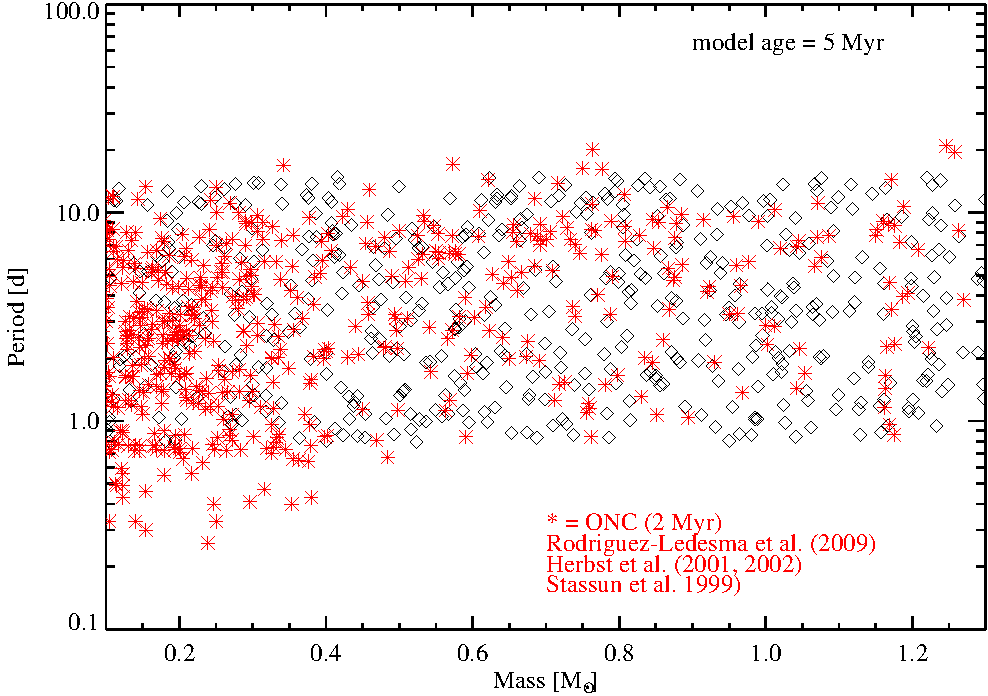
\includegraphics[width=\textwidth]{figures/introduction/matt_2015_fig2a.pdf}
  \end{minipage}
  \hfill
  \begin{minipage}[b]{0.5\textwidth}
    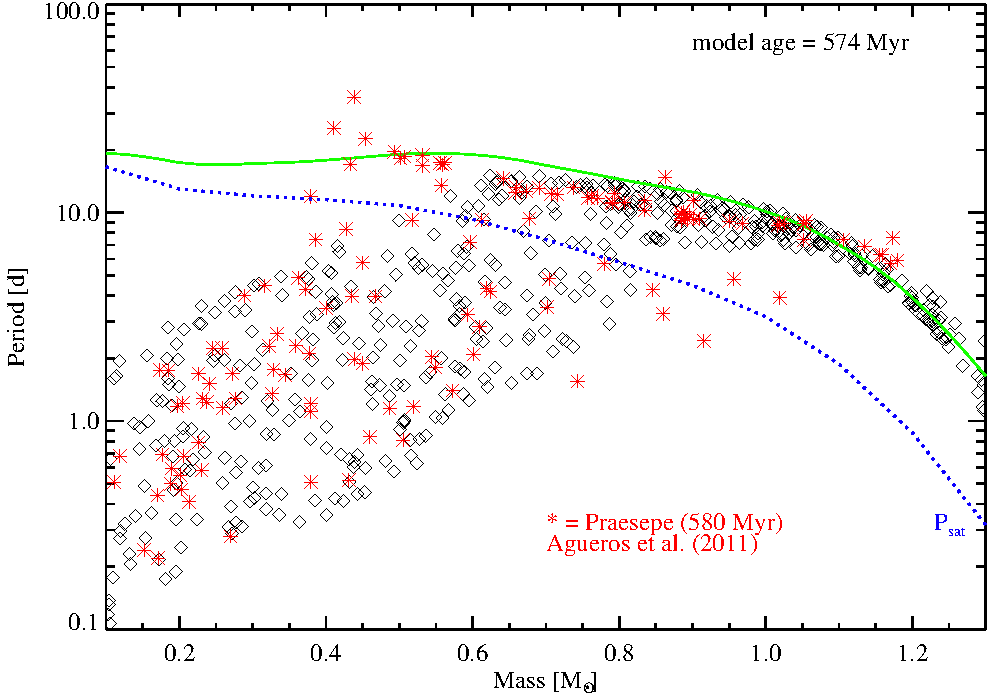
\includegraphics[width=\textwidth]{figures/introduction/matt_2015_fig2b.pdf}
  \end{minipage}
  \caption{From \citet{matt2015}.}
\end{figure}

Unfortunately, despite generally performing well, this model fails in a two key respects. Of primary concern to this work is the failure to reproduce observations at the short end of their available observations, a period of 


\section{Accretion in CVs}
\label{sect:introduction:accretion}
\todo{Proof read this, this is still a first draft.}
Accretion physics is important to the appearance and behaviour of a CV. While it is described briefly here,  more in-depth discussions can be found in \citet{warner1995} and \citet{hellier2001}.

When the donor star overfills its Roche lobe, matter is ejected from its surface at thermal velocities, $\sim 10 \rm km\ s^{-1}$ for a 5000K M dwarf, which is small when compared to the orbital velocity of the system. M dwarf velocities of $\sim 400-500 \rm\ km s^{-1}$ are common in the observations contained later in this work. Since the ejected material is effectively stationary as it leaves the donor, it falls along a ballistic trajectory towards the white dwarf primary and forms an accretion disc around it. 

Disc material gradually loses angular momentum and gravitational potential energy due to its viscosity, which acts over time to concentrate the majority of the disc's angular momentum in the minority of the disc's mass, effectively ejecting some material at high velocities at the expense of moving the remainder closer to the white dwarf. This viscosity partially arises from friction within the fluid of the disc, but the main source is thought to be from turbulence, random eddy currents moving material to different radii. This form of turbulence in a thin disc was formalised in the alpha disc model by \citet{shakura1973}, where viscosity, $\nu$, is related to scale height, $H$, and the speed of sound, $c_s$, by a free parameter, $\alpha$.

\begin{equation}
    \label{eqn:disc viscocity}
    \nu = \alpha c_s H
\end{equation}

Since turbulent eddies cannot be larger than $H$ or have velocities greater than $c_s$, $c_s H$ forms the upper limit of $\nu$, and $\alpha$ is limited in this model to values between 0 and 1. In typical CV accretion discs (i.e. quiescent discs, see \S\ref{sect:introduction:dwarf novae and superhumping}), $\alpha$ takes values from $\sim 0.01 - 0.05$ \citet{hellier2001}.

Material that enters the disc must lose gravitational potential energy before it can be accreted to the white dwarf surface. Approximately half of this energy is lost thermally, through radiating accretion light, and the other half is converted to the kinetic energy necessary to maintain orbit about the white dwarf at lower altitudes. This low orbit has typical velocities roughly an order of magnitude higher than the rotational velocity of the white dwarf, so for material to settle on the stars' surface, it must dissipate a large amount of kinetic energy. A region between the inner edge of the disc, and the surface of the white dwarf where this deceleration occurs is called the boundary layer, and can be a significant contributor to the total brightness of a CV. 



\section{CV variability and subtypes}
\todo{is this ok?}
The sections above have outlined the general structure and evolution of a CV, but not all systems are well described by this picture. CVs exhibit significant variability even on human timescales, often on the order of several magnitudes in brightness. Further, a few subtypes of CV exist that either lie significantly outside the normal evolutionary tracks we expect, or contain exotic components. These are briefly discussed, though the focus of this work is on ``classic'' CVs, and the majority of these subtypes are fundamentally incompatible with our analysis techniques.


\subsection{Magnetic CVs}
\label{sect:introduction:magnetic CVs}

It is possible for white dwarfs to have very strong magnetic fields, in the region of tens to hundreds of megagauss. Such white dwarfs are called polars, and are an interesting field of study in their own right, but when a polar is accreting material from a donor star the system is designated as an AM Her star. The intense magnetic field strength alters the CV evolution in a two main ways. The strong field lines of the polar mean that the hot, charged photosphere material transferred to the primary cannot form an accretion disc and instead falls directly onto the surface of the white dwarf. The impacting material forms a bright spot on its surface, which is usually bright enough to be visible from earth. In addition, the strong field lines force the white dwarf to become tidally locked to the donor star. 

There is also a subclass of magnetic CVs with weaker field strengths of a few megagauss, known as DQ Her stars. In these systems, the white dwarf is not tidally locked, and a partial disc can exist. However, as the existence of a disc is crucial to the characterisation technique used in this work (see \S WHAT\todo{Put in the relevant section here} for details), magnetic CVs are unsuitable for our analysis.

\subsection{Helium-rich CVs}
\label{sect:introduction:AM CVn}

A small number of CV donors are helium-rich, with much smaller radii than their hydrogen-rich counterparts; these can be semi-degenerate helium stars, the cores of highly evolved main sequence stars, or a second white dwarf. The  As a CV donor must be in contact with its Roche lobe, such systems are far more compact than usual, with orbital periods $\lesssim 65$ minutes. Such systems are AM CVn stars, after the prototypical system AM Canum Venaticorum. For further discussion on AM CVn stars, see \citep{solheim2010}.


\subsection{Classical Novae}
\todo{This section should also mention recurrent novae, briefly.}
The white dwarf in a CV is almost constantly accreting matter onto its surface. Over time this surface layer can build up, and get placed under immense pressure by the gravity of the white dwarf. Eventually, pressures rise enough to force material at the boundary to become degenerate, and once hot enough this boundary layer can begin nuclear fusion. 
Since the accreted material has become degenerate, it cannot expand in response to the extra energy from fusion and simply heats further, leading to more and more fusion and culminating in a complete detonation of the accreted material on the white dwarf's surface \citep{warner1995}. This detonation is finally able to overcome the surface gravity of the white dwarf, and the accreted material is blown from the surface.
These are generally one-off events, recognised by a significant brightening of the system of between 6 and 19 magnitudes, lasting anywhere from a few days, so several months. 

Once a system has experienced a classical nova, it is classified as a CNe system. \citep{warner1995}. However, theory suggests that all CVs experience classical novae many times over their lifetimes. The required amount of accreted material for the nova to occur depends on mass, but lies between $3\times10^{-5} M_\odot$ of hydrogen for a $1.3 M_\odot$ white dwarf, and $5\times10^{-3} M_\odot$ for a low mass, $0.6 M_\odot$ white dwarf \citep{hellier2001}. Typical CV accretion rates are around $10^{-9} M_\odot\ yr^{-1}$ for long period systems, and $10^{-10} M_\odot\ yr^{-1}$ for short period systems \citep{hellier2001, Pala2021}, suggesting classical novae recur at most every few million years, down to every few tens of thousands of years.

The amount of material retained by the white dwarf is likely negligible. Both population synthesis by \citep{wijnen2015} and observations by \citep{McAllister2017} indicate no evidence of mass growth over time for the white dwarfs in CVs, and hence that the expulsion of the accreted material in a classical nova is complete.

A final note is that some CVs show multiple classical novae in relatively quick succession \citep{schaeffer2010}. These Recurrent Novae (RNe) are distinguished by having more than one observed nova event recorded. As good quality data only exist for the last few centuries, this enforces a soft limit on recurrence interval of a few hundred years, though recent efforts have been made to search ancient records for candidate events \citep{hoffmann2022}. Only a handful of confirmed RNe are known; the variable star index \citep{Watson2006} only contains 11 systems classified as RNe.

\subsection{Dwarf Novae}
\label{sect:introduction:dwarf novae }

CVs also undergo less extreme brightening events, called Dwarf Nova (DN) outbursts. These brighten the system by between 2 and 5 magnitudes \citep{warner1995} and are more brief than typical CNe, lasting less than $\sim 20$ days. However, in contrast to CNe, they have recurrence times much more in line with human timescales, ranging from a few days to some decades. This is due to the fundamental difference in the physical origin of the two phenomena.

DN outbursts do not originate directly from either star in the system, but rather from the accretion disc around the white dwarf. Such outbursts are well-described by the disc instability model \citep{cannizzo1993, dubus2018}.

Initially, the disc is in a cooler, ``low'' state with low temperature, low surface density, and low viscosity. Material in the disc moves inwards due to friction from turbulence (see \S\ref{sect:introduction:accretion}) which is relatively weak in the low viscosity material, so radial movement of disc material is slow.

If the accretion rate of donor material exceeds the rate material falls onto the surface of the white dwarf, then a buildup of matter begins in the disc\todo{Unsure if I should talk about the outburst starting in an annulus, and spreading outwards from there? Seems irrelevant...}, raising the density and temperature. Eventually, this annulus reaches $\sim 7000K$, at which point hydrogen becomes partially ionised and a rapid further increase in temperature is triggered as the material becomes optically thick and heat is trapped in the disc. In addition, as the temperature and density rise, so does $c_s$, and following Equation~\ref{eqn:disc viscocity}, so does viscosity, even assuming constant $\alpha$. In fact, $\alpha$ {\it rises} during outburst, to $\alpha \sim 0.1 - 0.5$ \citep{hellier2001}. This hot, luminous, ``high'' state is again stable, and the disc is said to be in outburst. Now that the disc is more viscous, material is moved inwards more readily. The infall rate onto the white dwarf is much increased, and is now higher than the mass transfer rate, so the disc is drained onto the surface of the white dwarf. As it does so, the surface density and temperature begin to fall, and eventually protons and electrons recombine into hydrogen. While recombination is an exothermic process, the release of energy is outweighed by the material once again becoming optically thin and allowing radiation to more easily escape the disc. The disc now quickly cools back down to the quiescent, ``low'' state, returning to a low surface density, and the cycle can repeat itself. For a more in-depth look at this model, refer to discussions by \citet{cannizzo1993}, \citet{osaki1996}, \citet{warner1995}, \citep{hellier2001}, and \citet{Hameury2002}.

Three types of DNe exist, which exhibit somewhat different behaviour than what is outlined above. The first of which are SS Cyg stars, distinguished by very consistent amplitudes across outbursts, though there is variation in length, shape, and recurrence time.

Z Cam stars exhibit standstills, events where the system enters outburst, peaks in brightness, then begins to dim. However, rather than returning to its quiescent magnitude, the brightness is maintained $\sim 1-1.5$ magnitudes below peak brightness for a long period of time, typically between a few days, and a few years \citep{simonsen2014}.

The third subtype are SU UMa stars. These systems are known for their more complex behaviour, exhibiting superoutbursts and superhumping, and are described in \S\ref{sect:introduction:SU UMa}

\subsection{SU UMa stars}
\label{sect:introduction:SU UMa}

SU UMa stars are distinguished by exhibiting superoutbursts, similar to the regular outbursts that the star still undergoes, but with greater amplitudes and durations, but longer recurrence times. These outbursts are triggered by the disc radius growing to such an extent that it becomes tidally perturbed by the donor star, and turns elliptical. This can only take place for when the donor star is less than $\sim 1/3$ the white dwarf mass, so only short period systems see these superoutbursts. \citep{hellier2001}. 
SU UMa stars are also known for their superhumping, which also arises from the disc eccentricity. The tidal interaction between the disc and the donor produces an area of increased luminosity at the edge of the disc between the white dwarf and the donor \citep{warner1988}. As the disc is elliptical, the distance between this disc edge and the donor varies over the course of an orbit, causing a similar variation in brightness as the donor moves around the disc.
These fluctuations are called superhumps, and are useful as they provide a diagnostic to the mass ratio for the system as the  \citep{Patterson1998, Patterson2001, patterson2005}. 
\todo{This is terrible. Rewrite it.}Because of the strong influence of the donor, the disc is also subject to precession, with a precession rate slightly longer than the orbital period. The superhump period, $P_{\rm hump}$ is then a combination of the orbital period, $P_{\rm orb}$, and the precessional period $P_{\rm pr}$,
\begin{equation}
    \frac{1}{P_{\rm hump}} = \frac{1}{P_{\rm orb}} - \frac{1}{P_{\rm pr}}
\end{equation}
and can be readily observed with photometry from earth without the need for precise alignment that eclipse modelling requires. Since the precession period is dependant on the mass ratio and the disc radius, by finding the superhumping period of eclipsing CVs an empirical relationship can be found between the superhumping excess, $\epsilon$, and the mass ratio of a CV, where:
\begin{equation}
    \epsilon = \frac{P_{\rm hump} - P_{\rm orb}}{P_{\rm orb}}
\end{equation}
and several papers exist discussing and calibrating this relationship, see \citet{McAllister2019} for a recent calibration and good starting point for more information.


\subsection{Nova-like systems}

The disc instability model applies to CVs with mass transfer rates that are high enough to exceed the infall rate onto the CV during the ``low'' state, but low enough that the ``high'' state can still empty the disc. However, a subset of CVs have mass transfer rates high enough to sustain the high state and maintain a permanent outburst mode. Such systems are called Novalikes, or NL systems. Most NL CVs show little to no brightness variation, though a small number known as VY Scl stars do occasionally enter ``low'' states and dip in brightness by several magnitudes. \citet{livio1994} propose that this is triggered by a starspot rotating into the L1 point causing a fall in mass transfer rate. A precise mechanism here is not given, but since star spots are regions of concentrated magnetic fields, it is postulated that the stronger magnetic field of the spot disrupts magnetic braking in some fashion. A competing theory from \citet{wu1995} proposes that the fall in brightness is caused by the irradiation of the donor stars' atmosphere driving mass transfer, and that when this irradiation becomes blocked, the mass transfer rate falls enough for the disc to enter the low state for a short time.




\section{A modern understanding of AML}
% Here, put in some motivation about why we should try and understand AML in CVs - i.e. they are a good test bed since we can get so much information on their characteristics, and they're relatively simple systems. Understanding them is a good step towards larger and more complex phenomena.
A solid knowledge of exactly how and why CVs lose angular momentum has remained surprisingly elusive for several decades now. Early theories established gravitational waves and magnetic braking as the only two sources of AML \todo{ref}, but attempts to quantify this with evolutionary models \todo{ref} and population synthesis models \todo{ref} consistently fall short, as outlined in \S\ref{sect:introduction:AMLMechs}. Gravitational losses are well understood, and have been independently observed and studied, but the sources and consequences of magnetism in a stellar context is not so easy. CVs provide a testbed for probing magnetism in low mass stars that will be useful in other contexts. 

The missing source of AML is not necessarily magnetic in nature. 


Here are some links to papers that I should reference here.
\begin{itemize}
    \item \href{https://ui.adsabs.harvard.edu/abs/2020MNRAS.491.5717B/abstract}{Evidence for reduced magnetic braking}
    \item \href{https://iopscience.iop.org/article/10.3847/0004-637X/817/1/69}{THE INFLUENCE OF NOVA ERUPTIONS}
    \item \href{https://academic.oup.com/mnrasl/article/455/1/L16/2589619}{eCAML paper, schrieber 2016}
    \item \href{https://ui.adsabs.harvard.edu/abs/2021ApJ...914....5S/abstract}{Nova-produced Common Envelope: Source of the Nonsolar Abundances and an Additional Frictional Angular Momentum Loss in Cataclysmic Variables}
    \item \href{https://ui.adsabs.harvard.edu/abs/2018MNRAS.481.3604B/abstract}{The origin of magnetic fields in CV white dwarfs (2020)}
\end{itemize}

\subsection{The missing AML problem}
See the first year literature review for some content here. This subsection should quantify the missing AML problem with real observations and models, and tee up the next parts where some proposed solutions are discussed.

\subsection{Residual magnetic braking}

\subsection{Consequential AML}
also talk about empirical CAML, eCAML, here \citep{Schreiber2016}.

This will be very important! Lower mass donors will be able to accrete and retain less nova-processed material, so more will be lost from the system and carry with it more angular momentum. 
I think this dovetails with the lower mass white dwarf correlating with higher excess AML, since the same logic applies - the lower escape velocity from the system should allow more material to carry away angular momentum.
(https://ui.adsabs.harvard.edu/abs/2021ApJ...914....5S/abstract)

\section{Further issues with established CV models}

Population studies expect that up to 50\% of CVs should host a helium white dwarf \citep{politano1996}, though to date this has been notoriously difficult to test. 
\citet{zorotovic2010} examined a sample of post-common envelope binaries and found only $13\pm7\%$ of the sample to be expected to evolve into a CV containing a helium white dwarf. \href{https://arxiv.org/pdf/1609.06940.pdf}{On the white dwarf mass problem of CVs}

Additionally, observation and theory disagree on the white dwarf mass produced in CV evolution \citep{wijnen2015, liu2016, parsons2017}, with models predicting an excess of low-mass white dwarfs that are not observed. 
On top of this, there is the question of "do CVs grow in mass over time as they accrete?", to which the answer is no. 


Also, we expect there to be about 13\% of systems forming with a brown dwarf, which would put them below the period minimum -- which is not observed.

\href{https://articles.adsabs.harvard.edu/pdf/2010MmSAI..81..849R}{Ritter has some good points that I should include}

\section{Probing CV evolution}
The technique used for this thesis is primarily eclipse modelling, and MESA stellar evolution modelling, both of which are explained in detail in Chapter~\ref{chpt:modelling and techniques}

\subsection{$\epsilon - q$ relation for superhumpers}

\subsection{Donor mass-radius relation}
\todo{Essentially, Knigge 2011}

\subsection{Spectroscopy of the white dwarf}
\todo{Pala 2021 should be talked about here, along with whatever else you can dig up about spectroscopic analysis.}


\section{Closing remarks, and recap}



%\begin{figure}%[h!]
%\centering
%\includegraphics[width=14cm]{[YOUR PATH TO THE FIGURE_FOLDER/FIGURE.PNG]}
%\caption{}
%\label{introfig:sn_pectra}
%\end{figure}

%represent $70-75$percent of CCSNe \citep{eldridge13} and

